\documentclass{beamer}

\usepackage[utf8]{inputenc}
\usepackage[T1]{fontenc}
\usepackage{graphicx}
\usepackage{booktabs}
\usepackage{animate}

\usetheme{ulaval}

\title[Réseaux de neurones pour saisie automatique]{Réseaux de neurones profonds pour la saisie d'objets automatisée} 

\author{Alexandre Gariépy} 
\institute[ulaval] 
{
Université Laval \\
\medskip
\textit{alexandre.gariepy.2@ulaval.ca}
}
\date{\today}

\begin{document}

\begin{frame}
\titlepage
\end{frame}

\begin{frame}
\frametitle{Aperçu}
\tableofcontents 
\end{frame}

\section{Définition du problème}
\begin{frame}
  \frametitle{Définition}
  
\end{frame}

\begin{frame}
  \frametitle{Représentation à 5 dimensions}
  \begin{figure}
    \centering
    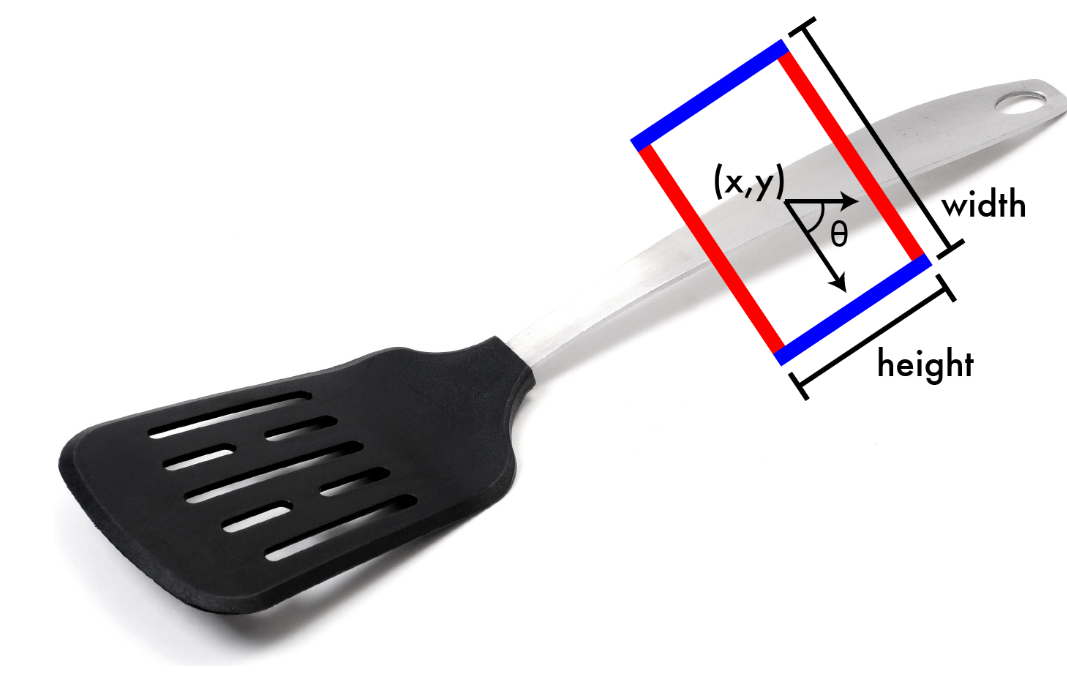
\includegraphics[width=0.8\textwidth]{img/grasp_rectangle.png}
    \caption{Représentation d'un point de saisie par un rectangle avec rotation}
    \label{fig:grasp_rect}
  \end{figure}
\end{frame}

\section{Réseau de neurones à convolution}
\begin{frame}
  \frametitle{Réseau AlexNet}
  \begin{figure}
    \centering
    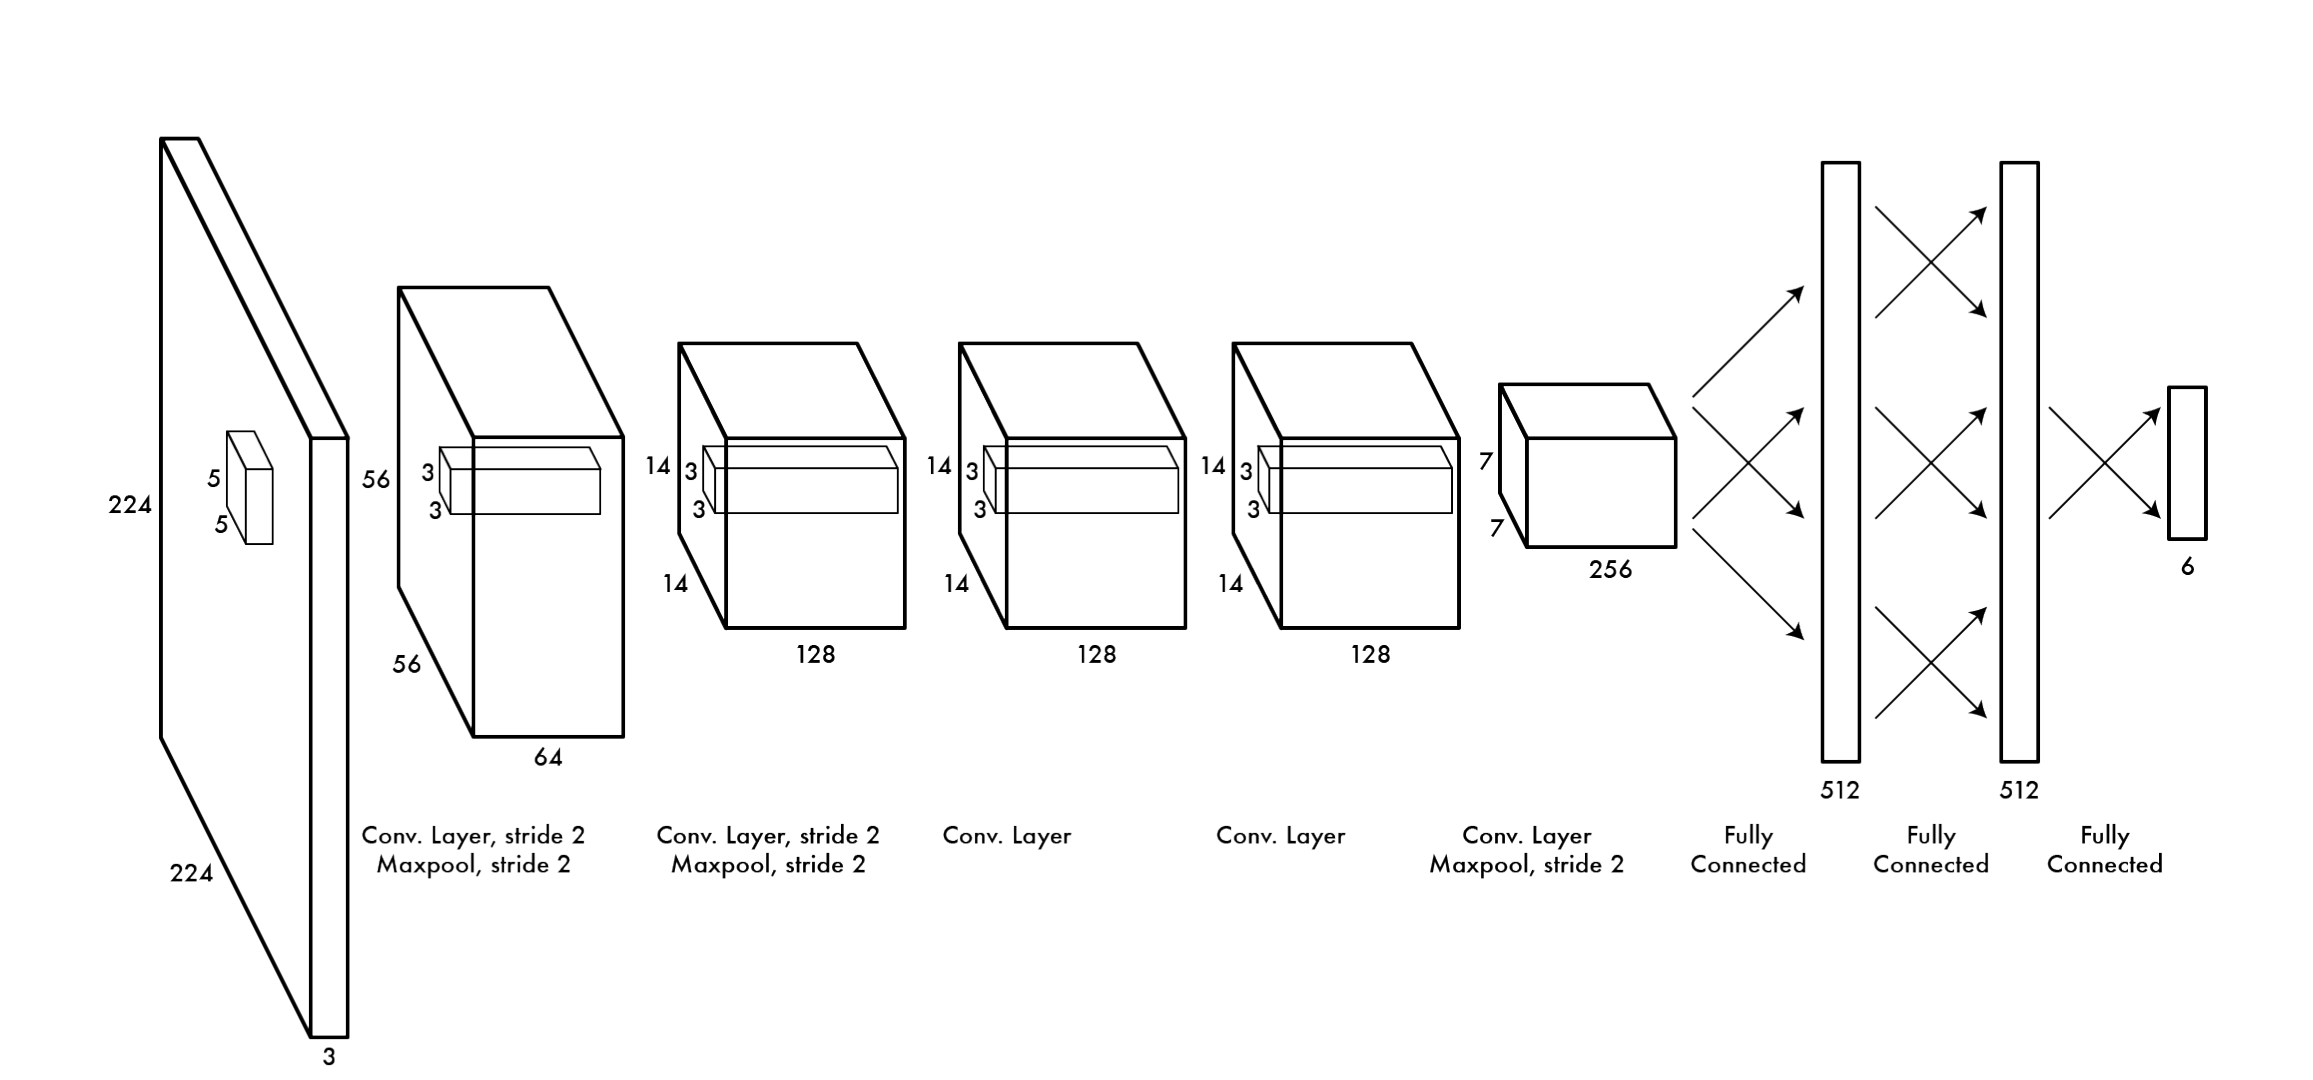
\includegraphics[width=0.9\textwidth]{img/alexnet.png}
    \caption{Architecture AlexNet}
    \label{fig:alexnet}
  \end{figure}
\end{frame}

\begin{frame}
  \frametitle{Convolution}
  \begin{center}
    \animategraphics[loop,width=0.6\linewidth]{1}{img/conv/img}{001}{021}
  \end{center}
\end{frame}

\begin{frame}
  \frametitle{Convolution}
  \begin{itemize}
  \item Réseau de convolutions: détecteur de particularités (\emph{features})
  \end{itemize}
  \begin{figure}
    \centering
    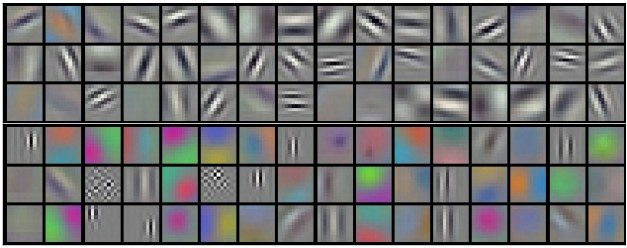
\includegraphics[width=0.6\textwidth]{img/weights.jpeg}
    \caption{Poids de la première couche du réseau}
    \label{fig:weights}
  \end{figure}
\end{frame}

\begin{frame}
  \frametitle{Couche de sortie}
  \begin{figure}
    \centering
    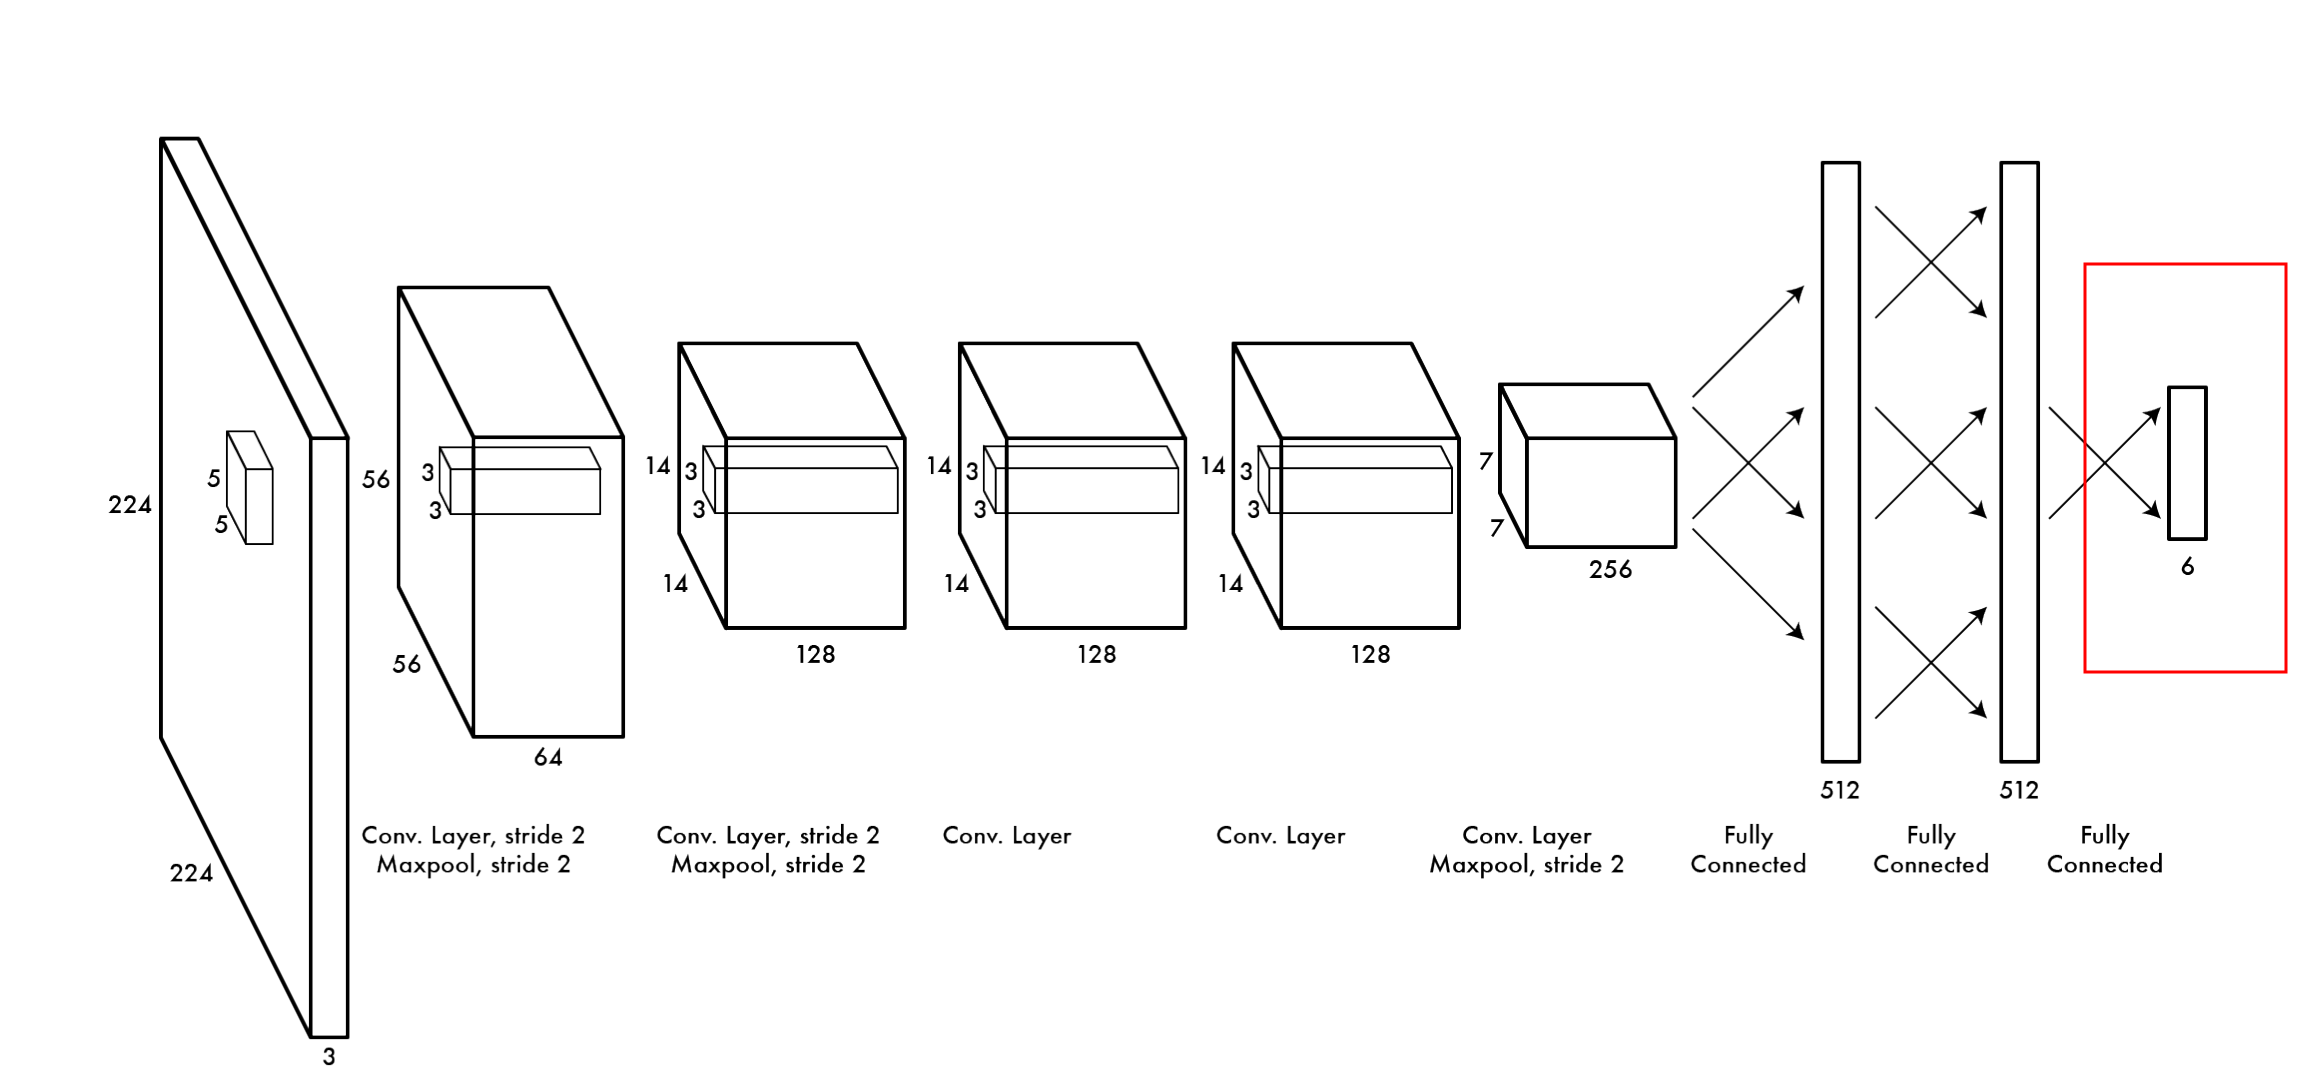
\includegraphics[width=0.9\textwidth]{img/last-layer.png}
    \caption{Couche de sortie du réseau}
    \label{fig:last_layer}
  \end{figure}
\end{frame}

\begin{frame}
  \frametitle{Couche de sortie}
  \begin{itemize}
  \item Encode la tâche à accomplir
  \item Évaluation de performance par la fonction de regret\footnote{\emph{loss function}}
  \item Correction de tous les poids par rétropropagation \footnote{\emph{back propagation}}
  \end{itemize}
\end{frame}

\section{Architectures pour la saisie d'objets}
\begin{frame}
  \frametitle{Jeu de données Cornell}
  1035 images RGBD de 280 différent objets dans 16 catégories
  \begin{center}
  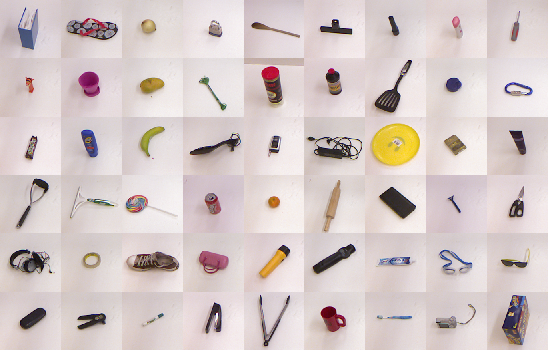
\includegraphics[width=0.75\textwidth]{img/cornell.png}
  \end{center}
\end{frame}

\begin{frame}
  \frametitle{Saisie directe}
  \begin{itemize}
  \item Prédiction directe d'un point de saisie
  \item 6 sorties: $[x, y, w, h, \sin(2\theta), \cos(2\theta)]$
  \item Suppression de symétries en utilisant $(\sin(2\theta), \cos(2\theta))$,
    entre -1 et 1
  \item \emph{loss} L2: $\sqrt{(x_{réel} - x_{prédit})^2 + (y_{réel} - y_{prédit})^2
    + ...}$
  \end{itemize}
  
\end{frame}

\begin{frame}
  \frametitle{Saisie directe + classification}
  \begin{itemize}
  \item Ajout d'une sortie: classe de l'objet
  \item Problème multi-objectif
  \item $Loss = \alpha Loss_{rectangle} + (1 - \alpha) Loss_{classification}$
  \item Intuition: production de \emph{features} spécialisées
  \end{itemize}
\end{frame}

\begin{frame}
  \begin{itemize}
  \item Généralisation de la saisie directe
  \item $N \times N \times 7$ sorties ($N = 7$)
  \item Un paramètre supplémentaire par rectangle: probabilité
  \end{itemize}
  \frametitle{Détection multiple (\emph{MultiGrasp})}
  \begin{figure}
    \centering
    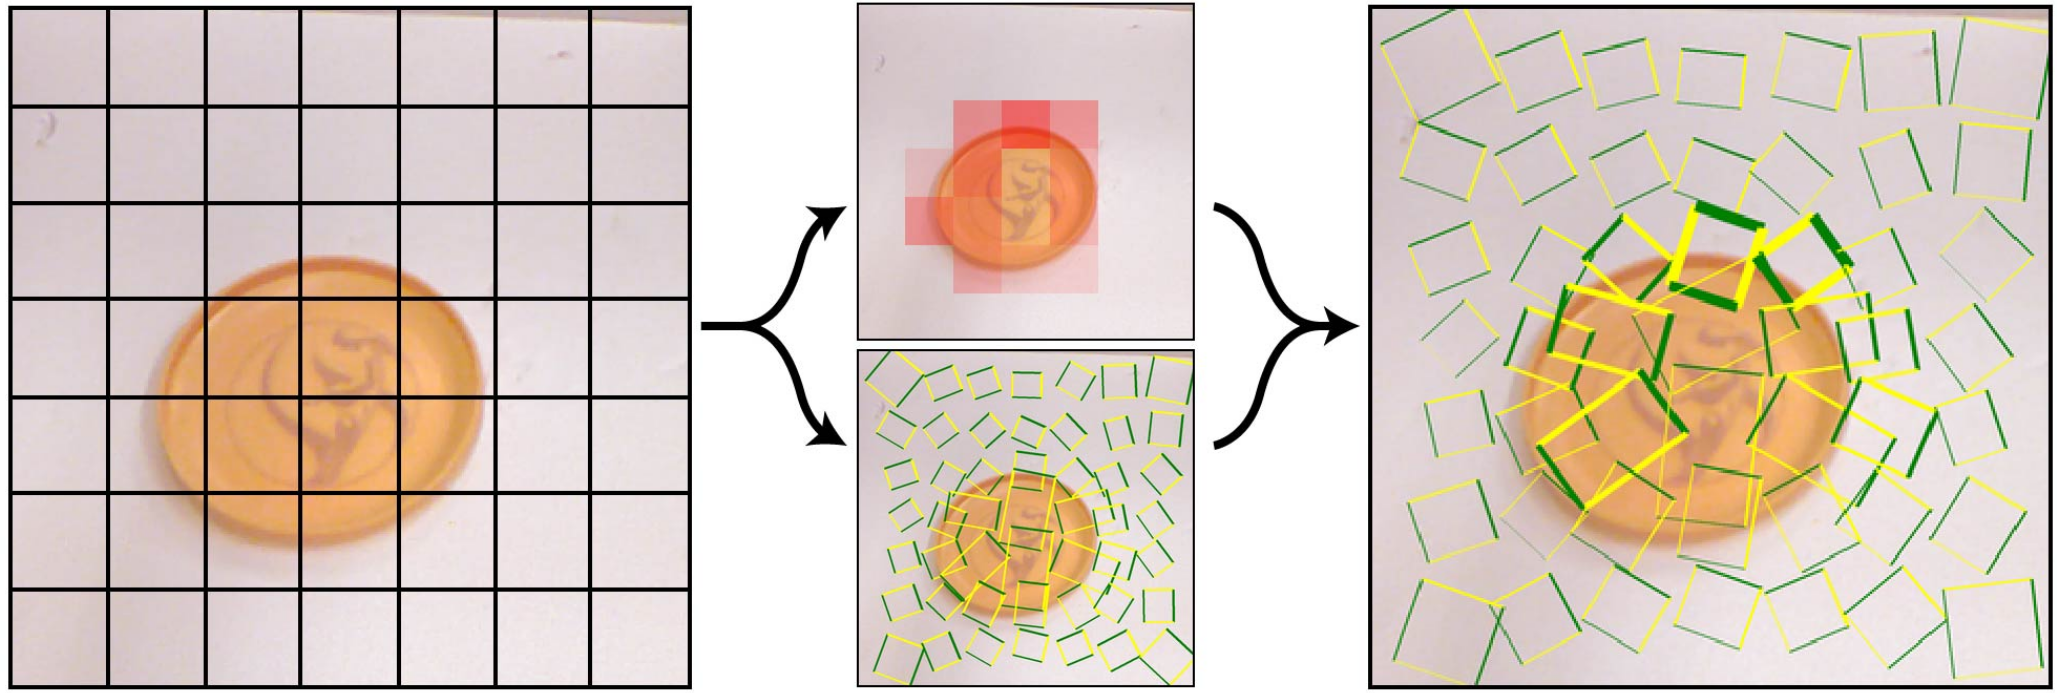
\includegraphics[width=0.8\textwidth]{img/multigrasp.png}
    \caption{Visualisation de la sortie \emph{MultiGrasp}}
    \label{fig:multigrasp}
  \end{figure}
\end{frame}

\section{Détails d'entraînement}
\begin{frame}
  \frametitle{Pré-entraînement}
  
\end{frame}

\section{Résultats}
\begin{frame}
  \frametitle{Métrique d'évaluation}
  
\end{frame}

\begin{frame}
  \frametitle{Résultats}
  
\end{frame}

\section{Questions}
\begin{frame}
  \frametitle{Questions}
  
\end{frame}

\begin{frame}
  \frametitle{\emph{Maxpool}}
  \begin{figure}
    \centering
    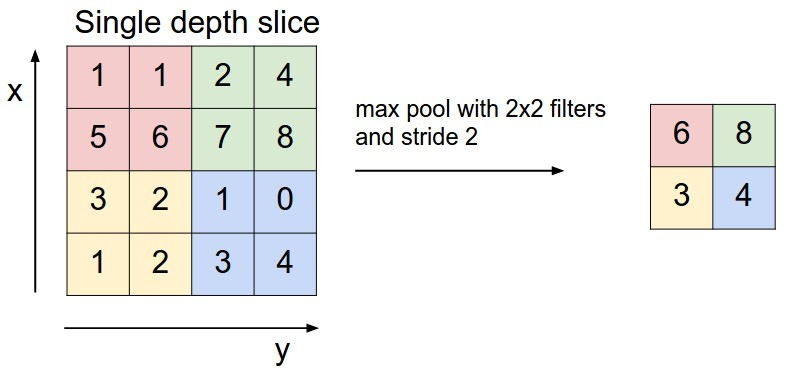
\includegraphics[width=0.8\textwidth]{img/maxpool.jpeg}
    \caption{Opération \emph{Maxpool}}
    \label{fig:maxpool}
  \end{figure}
\end{frame}

\end{document}
